% vim: set tw=78 sts=2 sw=2 ts=8 aw et ai:

\subsection{Artificial Neuron}
Artificial neural networks are inspired by the biological neural systems. The transmission of signals in biological neurons through synapses is a complex chemical process in which specific transmitter substances are released from the sending side of the synapse. The desire is to change the logical level of the receiving cell. 

\begin{figure}[H]
    \centering
    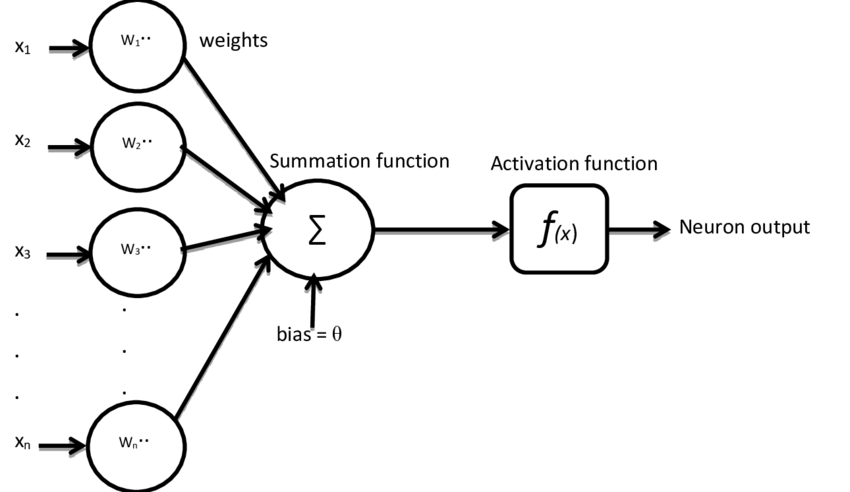
\includegraphics[width=0.7\linewidth]{img/artificialNeuron.png}
    \caption{Artificial neuron structural diagram\cite{impactANN}}
    \label{fig:artificialNeuron}
\end{figure}

The artificial neuron presented in the figure above has N inputs, each input being assigned a weight, denoted as $w_1, w_2...w_N$. The activation $y$ determines if the neuron is to be fired or not. It can be represented with the following formula:

\begin{equation}
    y=\sum_{i=1}^nw_ix_i
\end{equation}

\subsection{Neural network structure}
A neural network system consists of a varying number of artificial neurons and a very large number of interconnections. In a neural network, single neurons are arranged in layers. The manner in which they are arranged in a layer and how the connections are being executed with the next layer indicates the type of network in use. The three major important neural network types are:

\begin{itemize}
    \item Feed-forward of fully connected (FC) neural networks.
    \item Convolutional neural netrowks (CNNs)
    \item Recurrent neural networks (RNNs).
\end{itemize}

\begin{figure}[H]
    \centering
    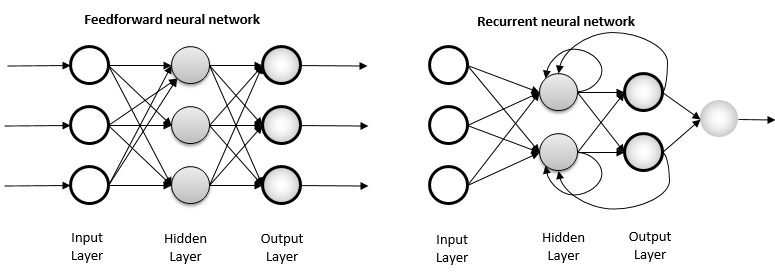
\includegraphics[width=0.8\linewidth]{img/feedForwardRecurrent.png}
    \caption{Examples of neural network architectures\cite{layersFigure}}
    \label{fig:layersFigure}
\end{figure}

In layered neural networks, the neurons are organized in the form of layers. The neurons in one layer get input from the previous layer and feed their output to the next layer. The layers which are processing the data are called hidden layers. The output layer is the last layer of a neural network and provides the results of a neural network. Usually, the output of a neural network is represented in the form of a probability of specific possible results. Each layer contained in a feed-forward layer is described by Equation (1), whilst the weight matrix $w_i$ contains an entry for each neuron connected between two layers. Networks with one or more hidden layers are called multi-layer networks.

\subsection{Inference and Training}

In most applications, ANNs are deployed in two phases. The first deployed stage is the training stage in which a known set of annotated data samples are used in order to create a model. When training, ANN models can be fine-tuned. When fine-tuning a model, weights of a previously-trained network are used to initialize the parameters of a new training. These weights may be adjusted for new constraints, such as a different dataset, reduced precision etc.

The second phase, known as inference, makes use of the learnt model to classify new data samples (i.e. inputs that were not previously seen by the model). In a typical setup, ANNs are trained and fine-tuned only once. The inference is implemented every time a new data sample needs to be classified. 